%% abtex2-modelo-projeto-pesquisa.tex, v-1.9.3 laurocesar
%% Copyright 2012-2015 by abnTeX2 group at http://abntex2.googlecode.com/ 
%%
%% This work may be distributed and/or modified under the
%% conditions of the LaTeX Project Public License, either version 1.3
%% of this license or (at your option) any later version.
%% The latest version of this license is in
%%   http://www.latex-project.org/lppl.txt
%% and version 1.3 or later is part of all distributions of LaTeX
%% version 2005/12/01 or later.
%%
%% This work has the LPPL maintenance status `maintained'.
%% 
%% The Current Maintainer of this work is the abnTeX2 team, led
%% by Lauro César Araujo. Further information are available on 
%% http://abntex2.googlecode.com/
%%
%% This work consists of the files abntex2-modelo-projeto-pesquisa.tex
%% and abntex2-modelo-references.bib
%%

% ------------------------------------------------------------------------
% ------------------------------------------------------------------------
% abnTeX2: Modelo de Projeto de pesquisa em conformidade com 
% ABNT NBR 15287:2011 Informação e documentação - Projeto de pesquisa -
% Apresentação 
% ------------------------------------------------------------------------ 
% ------------------------------------------------------------------------ 

\documentclass[
	% -- opções da classe memoir --
	12pt,				% tamanho da fonte
	openright,			% capítulos começam em pág ímpar (insere página vazia caso preciso)
	oneside,			% para impressão em verso e anverso. Oposto a oneside
	a4paper,			% tamanho do papel. 
	% -- opções da classe abntex2 --
	%chapter=TITLE,		% títulos de capítulos convertidos em letras maiúsculas
	%section=TITLE,		% títulos de seções convertidos em letras maiúsculas
	%subsection=TITLE,	% títulos de subseções convertidos em letras maiúsculas
	%subsubsection=TITLE,% títulos de subsubseções convertidos em letras maiúsculas
	% -- opções do pacote babel --
	brazil,				% o último idioma é o principal do documento
	]{abntex2}

% ---
% PACOTES
% ---

% ---
% Pacotes fundamentais 
% ---
\usepackage{lmodern}			% Usa a fonte Latin Modern
\usepackage[T1]{fontenc}		% Selecao de codigos de fonte.
\usepackage[utf8]{inputenc}		% Codificacao do documento (conversão automática dos acentos)
\usepackage{indentfirst}		% Indenta o primeiro parágrafo de cada seção.
\usepackage{color}				% Controle das cores
\usepackage{graphicx}			% Inclusão de gráficos
\usepackage{microtype} 			% para melhorias de justificação
% ---

%\usepackage[subentrycounter,seeautonumberlist,nonumberlist=true]{glossaries}

% ---
% Pacotes de citações
% ---
\usepackage[brazilian,hyperpageref]{backref}	 % Paginas com as citações na bibl
\usepackage[alf]{abntex2cite}	% Citações padrão ABNT

% --- 
% CONFIGURAÇÕES DE PACOTES
% --- 

% ---
% Configurações do pacote backref
% Usado sem a opção hyperpageref de backref
\renewcommand{\backrefpagesname}{Citado na(s) página(s):~}
% Texto padrão antes do número das páginas
\renewcommand{\backref}{}
% Define os textos da citação
\renewcommand*{\backrefalt}[4]{
	\ifcase #1 %
		Nenhuma citação no texto.%
	\or
		Citado na página #2.%
	\else
		Citado #1 vezes nas páginas #2.%
	\fi}%
% ---

% ---
% Informações de dados para CAPA e FOLHA DE ROSTO
% ---
\titulo{Um Motor de Jogos para Autoria de Aplicações de Hipermídia com NCLua}
\autor{Ivo Matheus de Goes Lopes}
\local{São Luís}
\data{2015}
\instituicao{%
  Universidade Federal do Maranhão -- UFMA
  \par
  Curso de Ciências da Computação
  \par
  Graduação}
\tipotrabalho{Trabalho de Conclusão de Curso}
% O preambulo deve conter o tipo do trabalho, o objetivo, 
% o nome da instituição e a área de concentração 
\preambulo{Uma experiência com Motores de Jogos com o fim de incentivar trabalhos com Ginga.}
% ---

% ---
% Configurações de aparência do PDF final

% alterando o aspecto da cor azul
\definecolor{blue}{RGB}{41,5,195}

% informações do PDF
\makeatletter
\hypersetup{
     	%pagebackref=true,
		pdftitle={\@title}, 
		pdfauthor={\@author},
    	pdfsubject={\imprimirpreambulo},
	    pdfcreator={LaTeX with abnTeX2},
		pdfkeywords={abnt}{latex}{abntex}{abntex2}{projeto de pesquisa}, 
		colorlinks=true,       		% false: boxed links; true: colored links
    	linkcolor=blue,          	% color of internal links
    	citecolor=blue,        		% color of links to bibliography
    	filecolor=magenta,      		% color of file links
		urlcolor=blue,
		bookmarksdepth=4
}
\makeatother
% --- 

% --- 
% Espaçamentos entre linhas e parágrafos 
% --- 

% O tamanho do parágrafo é dado por:
\setlength{\parindent}{1.3cm}

% Controle do espaçamento entre um parágrafo e outro:
\setlength{\parskip}{0.2cm}  % tente também \onelineskip

% ---
% compila o indice
% ---
\makeindex
% ---

% Novo list of (listings) para QUADROS

\newcommand{\quadroname}{Quadro}
\newcommand{\listofquadrosname}{Lista de quadros}

\newfloat[chapter]{quadro}{loq}{\quadroname}
\newlistof{listofquadros}{loq}{\listofquadrosname}
\newlistentry{quadro}{loq}{0}

% configurações para atender às regras da ABNT
\counterwithout{quadro}{chapter}
\renewcommand{\cftquadroname}{\quadroname\space} 
\renewcommand*{\cftquadroaftersnum}{\hfill--\hfill}

% ---
% Formatação de código-fonte
% ---
\usepackage{listings}

% Altera o nome padrão do rótulo usado no comando \autoref{}
\renewcommand{\lstlistingname}{Código}

% Altera o rótulo a ser usando no elemento pré-textual "Lista de código"
\renewcommand{\lstlistlistingname}{Lista de códigos}

% Configura a ``Lista de Códigos'' conforme as regras da ABNT (para abnTeX2)
\begingroup\makeatletter
\let\newcounter\@gobble\let\setcounter\@gobbletwo
  \globaldefs\@ne \let\c@loldepth\@ne
  \newlistof{listings}{lol}{\lstlistlistingname}
  \newlistentry{lstlisting}{lol}{0}
\endgroup

\renewcommand{\cftlstlistingaftersnum}{\hfill--\hfill}

\let\oldlstlistoflistings\lstlistoflistings
\renewcommand{\lstlistoflistings}{%
   \begingroup%
   \let\oldnumberline\numberline%
   \renewcommand{\numberline}{\lstlistingname\space\oldnumberline}%
   \oldlstlistoflistings%
   \endgroup}


\begin{document}

\selectlanguage{brazil}
\frenchspacing 

\imprimircapa
\imprimirfolhaderosto*

\pdfbookmark[0]{\listfigurename}{lof}
\listoffigures*
\cleardoublepage

\pdfbookmark[0]{\listtablename}{lot}
\listoftables*
\cleardoublepage

\pdfbookmark[0]{\listofquadrosname}{loq}
\listofquadros*
\cleardoublepage

\pdfbookmark[0]{\lstlistlistingname}{lol}
\begin{KeepFromToc}
\lstlistoflistings
\end{KeepFromToc}
\cleardoublepage

\begin{siglas}
  \item[GW] Ginga Wings
  \item[OO] Programação Orientada a Objetos
\end{siglas}

\pdfbookmark[0]{\contentsname}{toc}
\tableofcontents*
\cleardoublepage



\textual

\chapter{Introdução}

\chapter{Trabalhos Relacionados}

\chapter{Engine Ginga Wings}

\section{Arquitetura de Implementação}

Uma Engine de Jogos é um Software com o propósito de facilitar o desenvolvimento de jogos. Elas foram, a princípio, criadas para facilitar o desenvolvimento com estrutura similares – como por exemplo, a série de jogos de RPG intitulada Baldur’s Gate, da BioWare, que se utilizou da Infinity Engine –, deixando para o desenvolvedor apenas a preocupação de criar o jogo em si, e não perder metade do prazo do jogo construindo seu alicerce. A popularidade desse tipo de aplicação aumentou nos anos 90, com o aparecimento de jogos “mods” (nome dado a modificações de partes de um jogo, mas mantendo boa parte da estrutura) do famoso jogo Doom, criado pela Id Software. Isso foi possível graças à separação que a equipe fez entre os componentes do jogo – deixando bem definidos os códigos que controlavam o renderizador gráfico, a colisão de objetos, o sistema de áudio, os recursos de mídia e imagem, as regras de jogo, etc. -, o que permitiu que outros grupos de desenvolvedores modificassem apenas as partes que lhes interessava (basicamente os recursos de áudio e imagens, arquivos de armas, inimigos, fases, etc), utilizando-se de Toolkits liberados pela empresa. Hoje temos Engines bem mais genéricas do que as dos anos 90, que permitiam criar jogos de Doom. Engines como Unreal ou Unity podem ser utilizadas e modificadas para criar uma vasta variedade de jogos para várias plataformas, 3D e 2D. A Engine de Jogos Ginga Wings vem com uma proposta de trazer semelhante funcionalidade para aplicações de TV Digital que rodam o Middleware Ginga.

A GW é um Engine especializada em jogos com gráficos 2D e interação pelo controle remoto. Ela se utiliza de boa parte da API de NCLua - descrita pelo padrão de Sistema Brasileiro de TV Digital (ABNT 2007) – para prover funcionalidades através do Set-Top Box. Ela roda, inteiramente, com código Lua e se comunica com o Documento NCL nativamente, sendo essa uma de suas principais características. Apesar do desenvolvimento ser voltado para Set-Top Boxes, como o Ginga também roda em dispositivos móveis, a Engine pode ser utilizada para jogos nestes dispositivos.

\begin{figure}
\centering
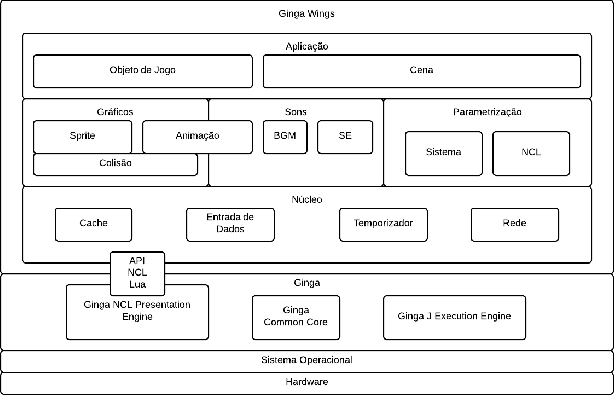
\includegraphics{arquitetura.png}
\caption{Arquitetura Ginga Wings}
\label{fig:arquiteturaGW}
\end{figure}

A visão geral da arquitetura da engine pode ser observada na Figura \ref{fig:arquiteturaGW}, com detalhamentos nas próximas seções.

\subsection{Hardware}

Hardware é onde a Aplicação está sendo executada. Geralmente será um Set-Top Box, mas pode ser um Dispositivo Móvel. Não é necessário detalhamento uma vez que a função do S.O. e do Middleware Ginga é deixar o tratamento do Hardware transparente.

\subsection{Sistema Operacional}

O Sistema Operacional é o principal sistema executado no Hardware, na maioria dos dispositivos. Normalmente em PCs, o SO se ocupa de gerenciar os recursos de Hardware, distribuindo-os para as aplicações. Por isso, em um PC, é de se esperar que nenhuma aplicação tenha total posse dos recursos de Hardware. Dispositivos Móveis e Set-Top Boxes, por outro lado, por terem uma função definida (contraposta ao SO de PC, que tem propósito geral), geralmente alocam praticamente todos os recursos à aplicação. A implementação de referência utiliza o Linux como Sistema Operacional padrão, pelo fato do mesmo ser um Software Livre.

\subsection{Ginga}

\begin{figure}
\centering
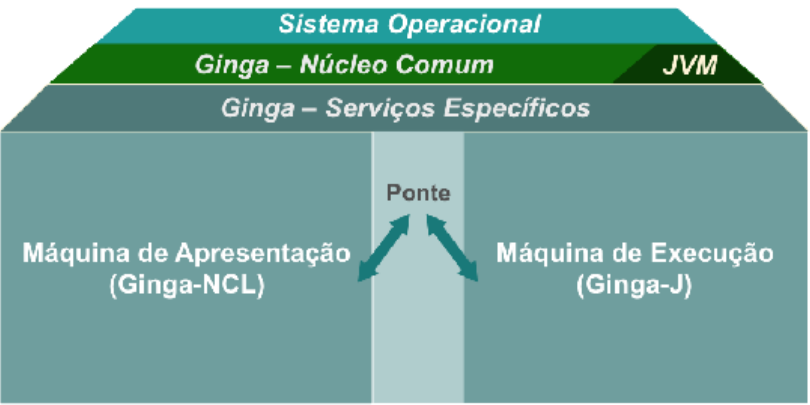
\includegraphics[scale=0.5]{ginga.png}
\caption{Visão Geral do Middleware Ginga}
\label{fig:ginga}
\end{figure}

O middleware é a camada de software que executa entre o sistema operacional e as aplicações. No caso específico do Sistema Brasileiro de TV Digital (SBTVD), o middleware Ginga foi desenvolvido. A Figura \ref{fig:ginga} apresenta uma visão geral da organização do Ginga. 

Como pode ser visto, ele é formado por diversos subsistemas, os quais foram implementados usando a linguagem C++. O núcleo comum do Ginga (CommonCore) implementa as funcionalidades principais do middleware, e acima dele temos uma camada de serviços específicos que consiste na implementação das APIs utilizadas pelas aplicações que executam sobre o middleware. Dois tipos de aplicações são suportadas pelo middleware brasileiro, as aplicações NCL (Ginga-NCL) e as aplicações Java (Ginga-J). Neste cenário, as aplicações acessam suas APIs específicas e estas APIs utilizam o núcleo comum para efetuarem suas operações. 

Em especial, ignoramos a Máquina de Execução em Ginga-J, e consideramos somente a de Apresentação, Ginga-NCL. Esta, em especial, possui o que chamamos de Objetos Imperativos NCLua, o que nada mais é do que a comunicação nativa existente entre o NCL e a Linguagem de scripting Lua. A criação, a ativação, pausa e encerramento do objeto NCLua são todos gerenciados a partir do NCL. 

O Middleware disponibiliza uma API que expõe métodos úteis para que o código Lua possa se utilizar dos recursos do sistema, tais como métodos para acesso aos pixels da tela reservada ao script, envio e recebimento de eventos e nós NCL, envio e recebimento de pacotes de rede pela internet, captura de entrada de dados da parte do usuário, entre outros. A Engine se baseia fortemente nestes métodos expostos para a implementação de suas funções.

\subsection{GingaWings}

Por fim, chegamos ao componente Ginga Wings. O primeiro nível da arquitetura é o grupo Núcleo, que possui os componentes Cache, Entrada de Dados, Temporizador e Rede. O componente Cache é responsável pelo gerenciamento básico de memória para sons, músicas e imagens, garantindo que um recurso não será várias vezes carregado na memória, e que recursos não utilizados pelo jogo sejam devidamente descartados da memória. O componente Entrada de Dados fornece várias formas de detecção de entrada do usuário, enriquecendo a API originada do Ginga. O componente Temporizador abusa da API de eventos do Ginga para garantir que o sistema será executado sempre em tempo constante. E por fim o componente de Rede oferece uma forma amigável de se enviar e receber pacotes via web.

\subsubsection{Gráficos}

\begin{figure}
\centering
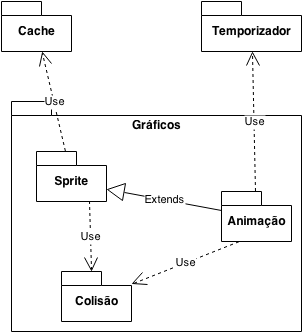
\includegraphics{diagrama_graficos.png}
\caption{Diagrama de Pacotes. Ginga Wings – Gráficos}
\label{fig:diagramaGraficos}
\end{figure}

O componente Gráficos pode ser detalhado pela Figura \ref{fig:diagramaGraficos}, na forma de pacotes. A estrutura básica do pacote é o Sprite. O Sprite é uma representação da posição, alargamento (zoom), e rotação de uma imagem, mas não é uma imagem em si. A imagem fica armazenada no Cache, de quem o Sprite depende. Um Sprite pode ter um objeto de Colisão associado a ele. A GW automaticamente detecta esta colisão e dispara eventos de caso este Sprite colida com outros. O pacote Animação é uma sequência de Sprites, gerenciada pelo Temporizador. Ela pode ter seu próprio objeto de colisão à parte do Sprite. A animação geralmente apenas muda qual Sprite está sendo exibido no momento, sendo a mudança gerenciada por um tempo t, o qual o Temporizador pode oferecer. A Animação também possui sua própria localização, alargamento e rotação à parte dos seus sprites.

\subsubsection{Audio}

\begin{figure}
\centering
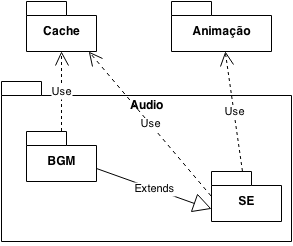
\includegraphics{diagrama_audio.png}
\caption{Diagrama de Pacotes. Ginga Wings – Audio}
\label{fig:diagramaAudio}
\end{figure}

O componente Audio, conforme ilustrado na Figura \ref{fig:diagramaAudio}, também possui dependência com o Cache. Diferentemente do que ocorre com imagens, não há uma exposição de métodos para manipulação de sons diretamente. Por isso é preciso utilizar-se de eventos NCLua para que algum som seja tocado através do Documento NCL, não do código Lua. O objetivo do Cache neste caso é gerar estes eventos. Mais detalhes na seção de API. Existem dois tipos de Áudio, BGM e SE. BGM signifca Backgroung Music, ou música de fundo. Basicamente são músicas que tocam em loop infinito enquanto o jogador manipula o jogo. SE significa Sound Effects, ou Efeitos Sonoros, que são podem ser descritos como Onomatopeias na gramática. As SEs são utilizadas pelas Animações para tocar sons sincronizados.

\subsubsection{Parametrização}

\begin{figure}
\centering
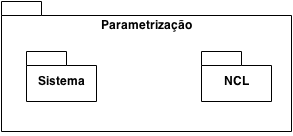
\includegraphics{diagrama_parametrizacao.png}
\caption{Diagrama de Pacotes. Ginga Wings – Parametrização}
\label{fig:diagramaParametrizacao}
\end{figure}

O componente Parametrização é uma das principais características do sistema: permite que o usuário de um Documento NCL envie parâmetros para o código Lua, configurando e controlando o jogo a partir do próprio NCL. Utilizando-se de estruturas como Âncoras e Links, é possível criar uma Engine Básica de jogos e orientá-la totalmente pelo seu código NCL: por exemplo, é possível definir uma fase inteira de Super Mario World utilizando NCL e NCLua. O código Lua teria a Engine básica, com os eventos, cenários, comportamentos de inimigos e itens, etc, enquanto que o código NCL seria o responsável por dizer como a fase seria desenhada, quais inimigos aparecem nela, e onde aparecem. Ele pode utilizar âncoras para determinar o fim de jogo caso o tempo termine, e por aí vai. É preciso, no entanto, que o código Lua esteja pronto para receber e interpretar estes parâmetros. A parametrização NCL captura esses parâmetros e os envia para dentro do código Lua, onde classes especializadas devem estar prontas para recebe-los e processá-los. A parametrização de Sistema possui toda e qualquer configuração geral do jogo: qual a resolução base que ele executa, FPS aceitável, entre outras configurações. 

\subsubsection{Aplicação}

\begin{figure}
\centering
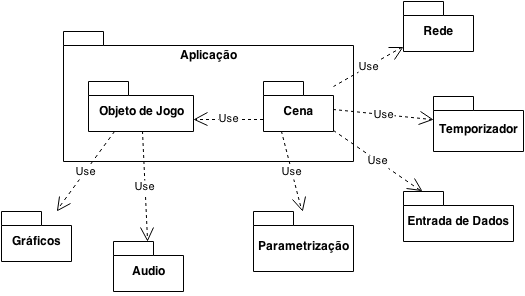
\includegraphics{diagrama_aplicacao.png}
\caption{Diagrama de Pacotes. Ginga Wings – Aplicação}
\label{fig:diagramaAplicacao}
\end{figure}

Por fim temos o componente de Aplicação, que utiliza todos os outros componentes. Seu principal pacote é a Cena, que junta os componentes de Entrada de Dados, Temporizador, Rede e Parametrização em um só lugar. O Temporizador determina, neste pacote, quantas vezes ele será atualizado por segundo. A Cena não interage diretamente com Músicas e Imagens, agindo através de Objetos de Jogo, estes sim, que encapsulam toda a estrutura de Mídia. 

\section{Detalhamento da API}

\subsection{Class}

A criação de jogos geralmente envolve códigos grandes e complexos. Claro, alguns jogos mais simples podem ter apenas algumas dezenas de linhas de código os definindo completamente, desde a aplicação gráfica, a entrada de dados e as respostas do jogo. Porém, para a maioria dos casos um jogo é uma série de códigos grande e complexa. Com o crescimento de qualquer tipo de código, sua manutenção tende a ficar cada vez mais complicada. Uma solução para isto é OO, que permite uma maior organização do código ao agrupar o funcionamento do sistema em objetos, suas possíveis ações e seus relacionamentos com outros objetos. Com isto em vista, tornou-se uma necessidade a implementação de tal funcionalidade, já que Lua não dá suporte a OO, sendo na verdade uma linguagem de protótipos.


\begin{lstlisting}[caption={Exemplo de Criação de Classe},label=cod_class_1,frame=single]
1.	GW_Codes.classes.Block = {}
2.	GW_Codes.classes.Block.superclass = "OBJECT"
3.	function GW_Codes.classes.Block:init()
4.		GWClasses.Block().__superclass().init(self)
5.	end
\end{lstlisting}


O propósito do módulo \verb|Class| é emular a funcionalidade de classes de OO, permitindo definir uma classe, criar instâncias dela, e também ter herança não múltipla. É extremamente fácil criar uma classe utilizando este módulo, como mostra o exemplo no Código \ref{cod_class_1}.

Lua funciona utilizando tabelas e metatabelas, que são os objetos nativos responsáveis por emular o funcionamento de classes para a GW. A linha 1 cria uma tabela que armazenará a estrutura da classe \verb|Block|. A segunda linha define qual é a classe pai da classe \verb|Block|. No caso, a classe \verb|OBJECT|, que é a classe padrão, já implementada na GW, que disponibiliza todas as funcionalidades básicas da GW. Todas as classes devem herdar de \verb|OBJECT|. É possível trabalhar sem ela, porém será mais difícil tirar proveito do que a GW tem a oferecer. A linha 3 define uma função que é inicializada toda vez que um objeto dela é instanciado. A linha 4 faz o equivalente a super em linguagens orientadas a objeto, permitindo que a classe pai inicialize seus atributos e métodos junto com a inicialização da classe filha. A passagem do parâmetro self é obrigatória para que a classe pai possa alterar a metatabela da filha. A linha 5 termina a função.

Para criar uma instância da classe \verb|Block|, basta chamar o método new.

\begin{lstlisting}[caption={Instanciando uma Classe},label=cod_class_2,frame=single]
1.	GW_Classes['Block'].new()
\end{lstlisting}

O método criará uma instância da classe \verb|Block| e passará a referência para a variável block. A tabela \verb|GW_Classes| guarda uma referência para todas as classes instanciáveis – a exemplo, a classe \verb|OBJECT|. O nome da classe será igual ao passado para a variável \verb|GW_Codes| no Código \ref{cod_class_1}. 

\subsubsection{Class:\_\_class() : table}

Retorna a estrutura de classe do objeto em questão.

\subsubsection{Class:\_\_classname() : String}

Retorna o nome da classe do objeto.

\subsubsection{Class:\_\_superClass() : metatable}

Retorna a estrutura de classe da classe pai do objeto.

\subsubsection{Class:\_\_is\_a(string: nomedaclasse) : boolean}

Verifica se o objeto é da mesma classe que a informada no parâmetro. Neste caso, verifica se os nomes são iguais.

\subsubsection{Class:\_\_is\_a(table: classe) : boolean}

Verifica se o objeto é da mesma classe que a informada no parâmetro. Neste caso, verifica se a metatable é igual à metatabela de classe do objeto.

\subsubsection{Class:\_\_respond-to(string: método) : boolean}

Verifica se o método passado existe na classe em questão. Por ser uma tabela simulando uma classe, é possível que um objeto tenha mais funções visíveis do que a classe disponibiliza. Estas funções não são inspecionados por esta função.

\subsection{Game\_Object}

Como mencionado, existe uma classe base, chamada simplesmente de OBJECT. Ela disponibiliza as funções básicas da GW, por isso é recomendado que qualquer objeto de jogo herde desta classe. Um objeto que herde de OBJECT automaticamente terá acesso a disparadores de eventos (por exemplo, disparar um evento quando um objeto Block tocar em outro), terá acesso a um comportamento, invocado automaticamente, desenho na tela, automático, funções de acesso à rede e de destruição do objeto. A classe objeto dá a seus filhos acesso a um sprite, uma posição na tela, e uma tabela de variáveis locais.

\subsubsection{Object:update() : boolean}

É a função principal da classe, chamando sua função de comportamento, gerenciando seus eventos e também o desenhando na tela. Caso o objeto tenha sido desposado, não realiza nenhuma dessas ações. Retorna true caso consiga realizar todas as suas operações.

\subsubsection{Object:dispose() : boolean}

Desposa um objeto, ou seja, este objeto não será mais considerado como ativo pela GW. Retorna true caso consiga desposar o objeto.

\subsubsection{Object:draw()}

Desenha o objeto na tela. 

\subsubsection{Object:\_\_create\_event(string: event)}

Cria um evento como o nome event. O evento criado é uma tabela, que possui a entrada command, uma função que é executada quando o evento é disparado, e outra entrada result, que guarda o resultado do evento gerado para que possa ser devidamente tratado. 

\subsubsection{Object:\_\_consume\_event(string: event)}

Faz uma chamada à entrada command do event parâmetro caso ele tenha sido disparado. Retorna true caso tenha sucesso. Deve ser invocado por funções interessadas em obter uma funcionalidade do evento, por exemplo, um objeto Gato iria chamar o evento Rato:\_\_consume\_event(‘saiu\_da\_toca’) e ler, em seguida, Rato.events[‘saiu\_da\_toca’] para verificar se o rato saiu da toca para que ele possa então caçá-lo. Um evento pode ser consumido até que reinicie o loop. O método command é invocado todas as vezes, portanto é preciso ser cauteloso ao codifica-lo.

\subsubsection{Object:\_\_\_\_fire\_event(string: event)}

Dispara o evento event. Todos os objetos que invocarem a função \_\_consume\_event() poderão obter os dados do evento gerado. Deve ser chamado pelo próprio objeto. Aproveitando o exemplo do gato e do rato, é o objeto rato que define Rato.\_\_fire\_event(‘saiu\_da\_toca’), para que enfim o gato possa invocar o método \_\_consume\_event() e correr atrás do rato fujão.

\subsection{Timer}

Este módulo, Game\_Timer, é o responsável por controlar os eventos temporais na aplicação. Ela armazena o tempo geral da aplicação, a taxa de frame rates (que determina quantas vezes por segundo a tela é renderizada, e portanto, o sistema é atualizado) esperada pela aplicação, e o tempo entre um loop e outro. Por padrão, a taxa de frame rates é 20, tendo em vista que o Set-Top Box não foi projetado para rodar aplicações pesadas, e o olho humano conseguir distinguir imagens fluídas em até 18 frames por segundo. Por causa disso não é possível criar animações muito fluídas sob a configuração padrão. Ela pode ser alterada de acordo com as necessidades do usuário, porém a performance do sistema como um todo deve ser levada em consideração. 

\subsubsection{Game\_Timer:sync(number: total\_time) : number}

Existem duas maneiras de se programar eventos temporais com frame rate: utilizando o frame rate como unidade de tempo; e utilizando o frame rate como medida de tempo. O primeiro cria uma estrutura temporal Dependente do Frame Rate (DFR). Se a taxa de frames for normal (usemos nosso exemplo de 20 frames por segundo), a aplicação irá executar em velocidade normal. Se, por algum motivo, a aplicação contiver um processo pesado e o frame rate cair para 10, a aplicação irá rodar duas vezes mais lento. Por outro lado, caso a aplicação receba atenção total do processador e conseguir rodar a 30 frames, o jogo irá rodar mais rápido. A segunda maneira, mais conhecida como Jogo em Tempo Real ou Independente de Frame Rate (IFR), se utiliza do intervalo entre cada loop do temporizador para calcular quanto tempo realmente passou, atualizando todos os objetos de jogo de acordo com o tempo passado. Desta forma, o jogo mantém sua velocidade de execução mesmo com a variação de frames por segundo – que por outro lado gera “paralizações” no jogo, geralmente chamadas de lag. Por outro lado, algumas aplicações ficam mais complexas, por exemplo, a detecção de colisão – é necessário realizar previsões dos movimentos dos objetos da cena para verificar se eles colidiram durante o intervalo de tempo. Com o devido cuidado, ambas as formas de manipular o tempo são viáveis, e o GW dá suporte a ambas.

\begin{lstlisting}[caption={Exemplo de uso da função sync},label=cod_timer_1,frame=single]
1.	pixels = Game_Timer:sync(20) --pixels = 20
\end{lstlisting}

A DFR é como a GW funciona normalmente. Para se trabalhar com a IFR, existe esta função no módulo Timer. Ele recebe um tempo e infere o quanto passou dele no intervalo entre os frames. O parâmetro deve indicar o movimento, através do tempo, por 1 segundo, sob o qual o método vai trabalhar. Por exemplo, se o Herói do jogo se movimenta a 20 pixels por segundo, em um jogo rodando a 20 FPS (frames por segundo), com a aplicação desta função, ele andará 1 pixel por segundo, a cada frame. Se por algum motivo a velocidade do jogo cair para 14 FPS, a velocidade do Herói será de 1.42 pixels por segundo.

\subsection{Graphics}

Módulo responsável pela renderização dos gráficos na tela. É possível informar uma ordem para que a renderização seja realizada. A GW possui uma resolução, nativa, que deve ser informada para o módulo. O jogo é renderizado na resolução nativa e após a renderização, se ajusta ao tamanho da tela da TV.

\subsubsection{Game\_Graphics:insertLayer(number: n, table: obj)}

Caso o objeto obj possua o método draw, que é chamado para realizar a renderização do mesmo, ele é incluído na lista de objetos a serem renderizados pelo módulo. Objetos com um n menor são desenhados primeiro, portanto os que tiverem os maiores valores ficarão por cima no resultado final. Não há garantia de ordenação para objetos com valores n iguais.

\begin{lstlisting}[caption={Definindo a ordem de renderização para a classe Board},label=cod_graphics_1,frame=single]
1.	GW_Codes.classes.Board.drawLayer = 1
2.	Game_Graphics:insertLayer(4, board)
\end{lstlisting}

Para setar um valor n padrão para todos os objetos de uma classe, basta seguir o exemplo no Código \ref{cod_graphics_1}, linha 1. Valores individuais podem ser aplicados, também, como mostrado na linha 2.

\subsection{Sprite}

Módulo básico, que armazena as gráficos da aplicação. Dá suporte tanto a gráficos estáticos quanto animados. Possui também suporte para física básica, na forma de colisões.

\subsubsection{Sprite.new(string: path) : table}

Cria uma instância da classe Sprite com a imagem referenciada pelo caminho path. Caso não encontre a imagem cria uma Sprite sem imagem. O Sprite criado não é subdividido, tem animação ativado (mas não executa nenhuma), e tem uma área de colisão de acordo com o tamanho da imagem.

\subsubsection{Sprite:set\_crop(number: w, number: h)}

Determina em quantos pedaços a imagem será repartida. Esta partição não altera o arquivo de imagem utilizado pelo Sprite, apenas determina pedaços de tamanho igual para serem desenhados com a função draw(). Qual parte será renderizada deve ser determinada pelo atributo anim\_index. O index é definido a partir do número de linhas e colunas. Por exemplo, se $w = 4$ e $h = 4$, o $index = 9$ representará a parte da imagem localizada na linha 3, coluna 1.

\begin{lstlisting}[caption={Exemplo de uso da função set\_crop},label=cod_sprite_1,frame=single]
1.	board = Sprite.new("board.png");
2.	board:set_crop(4,4)
3.	board.anim_index = 6
\end{lstlisting}

\subsubsection{Sprite:setup\_frames(number: index, number: steady, string: sound, table: offset)}

Permite configurar um frame de animação para o Sprite.  Index informa qual o índice da animação (os frames são organizados de acordo com esse índice); steady informa quantos milissegundos o frame permanecerá ativo (valores muito baixos podem tornar o frame quase indistinguível, valores muito altos pode “paralisar” a animação); sound informa que o frame deve tocar o som informado pelo campo no início do frame. Um valor vazio ou nulo terão o mesmo efeito, sem som. Offset é uma tabela, com valores x e y, indicando que o Sprite deve mover sua imagem mas sem mover a matriz. Ou seja, a imagem renderizada vai mudar sua posição de pintura na tela, mas o objeto Sprite manterá sua posição original.

\begin{lstlisting}[caption={Exemplo de uso da função setup\_frames},label=cod_sprite_2,frame=single]
1.	board = Sprite.new("board.png");
2.	board:setup_frames(0, 4, null, {x=0, y=0})
\end{lstlisting}

\subsection{Cache}

Módulo responsável por gerenciar os recursos de mídia da aplicação. Gerencia tanto recursos de áudio como de imagem. O gerenciamento de imagens é automático, porém o de áudio, por depender do NCL para ser feito, precisa de configurações mais cuidadosas.

\subsubsection{Game\_Resources.load\_image(string: path)}

Carrega a imagem referenciada no caminho path na memória e retorna uma referência para ela. Chamadas posteriores a este mesmo path apenas retornarão uma referência. Alterações no arquivo de imagem, portanto, afetarão todos os objetos que chamarem a referenciarem.

\subsubsection{Game\_Resources.load\_background(string: path)}

Invoca um recurso de imagem do caminho padrão “media\textbackslash backgrounds\textbackslash”. É um método auxiliar com a única finalidade de facilitar a obtenção de recursos de imagem.

\subsubsection{Game\_Resources.load\_character(string: path)}

Invoca um recurso de imagem do caminho padrão “media\textbackslash characters\textbackslash”. É um método auxiliar com a única finalidade de facilitar a obtenção de recursos de imagem.

\subsubsection{Game\_Resources.free\_image(string: path)}

Informa ao Cache que a imagem em path deve ser liberada da memória. O Cache vai registrar o pedido, porém a imagem só será removida se todos os recursos que pediram a imagem o liberarem.

\subsubsection{Game\_Resources.play\_SE(string: label)}

Envia uma requisição ao NCL para tocar o áudio label. SE é a sigla para Sound Effects (Efeitos Especiais). SEs são geralmente utilizadas para representar sons ambientes e de HUDs / sistema (Head Up Display, como geralmente são chamadas as telas de interface do jogo, como status, vida, dinheiro, etc). Uma configuração especial para este tipo de som deve ser provida pelo arquivo .ncl que chamada o script do GW.

\subsubsection{Game\_Resources.stop\_SE(string: label)}

Envia uma requisição ao NCL para parar o áudio label. Uma configuração especial para este tipo de som deve ser provida pelo arquivo .ncl que chamada o script do GW.

\subsubsection{Game\_Resources.pause\_SE(string: label)}

Envia uma requisição ao NCL para pausar o áudio label. Uma configuração especial para este tipo de som deve ser provida pelo arquivo .ncl que chamada o script do GW.

\subsubsection{Game\_Resources.play\_BG(string: label)}

Envia uma requisição ao NCL para tocar o áudio label. BG é a sigla para Background Sound (Sons de fundo), ou seja, canções que ficam tocando, em loop, enquanto a aplicação executa. Quando a canção termina sua execução ela é iniciada novamente, criando um loop. Uma configuração especial para este tipo de som deve ser provida pelo arquivo .ncl que chamada o script do GW.

\subsubsection{Game\_Resources.stop\_BG(string: label)}

Envia uma requisição ao NCL para parar o áudio label. Uma configuração especial para este tipo de som deve ser provida pelo arquivo .ncl que chamada o script do GW.

\subsubsection{Game\_Resources.pause\_BG(string: label)}

Envia uma requisição ao NCL para pausar o áudio label. Uma configuração especial para este tipo de som deve ser provida pelo arquivo .ncl que chamada o script do GW.

\subsection{Scene}

Módulo que centraliza e controla todos os outros. Os Game\_Objects devem ser manipulados junto com a lógica do jogo, utilizando este módulo. Uma instância do GW só tem 1 objeto Scene, que deve gerenciar os vários recursos. 

\subsubsection{GWScene:begin()}

Esta função deve ser utilizada para inicializar todos os objetos da aplicação que rodarão junto com a scene.

\begin{lstlisting}[caption={Exemplo de uso da função begin},label=cod_scene_1,frame=single]
1.	function GWScene:begin()
2.		self.vars.color = 'red'
3.		self.vars.board = GWClasses['Board'].new()
4.		self.vars.score = GWClasses['Score'].new()
5.		table.insert(self.objects, self.vars.board)
6.		Game_Graphics:insertLayer(self.vars.board.
			drawLayer, self.vars.board)
7.		table.insert(self.objects, self.vars.score)
8.		Game_Graphics:insertLayer(self.vars.score.
			drawLayer, self.vars.score)
9.		GW_Codes.classes.Block.createBlocks()
10.		self:createToy()
11.		Game_Resources.play_SE('playback')
12.	end
\end{lstlisting}

\subsubsection{GWScene:behavior()}

Esta função determina o comportamento da Scene, e as interações entre os objetos. A lógica de comportamento interna do objeto não deve ser implementada aqui. O consumo de eventos, do Game Object, deve ser aplicado aqui.

\begin{lstlisting}[caption={Exemplo de uso da função behavior},label=cod_scene_2,frame=single]
1.	function GWScene:behavior()
2.		if self.vars.toy:__consume_event('endGame') then
3.			self:End()
4.		end
5.		if self.vars.toy:__consume_event('gotFired') then
6.			self:deleteObject(self.vars.toy)
7.			self:createToy()
8.		end
9.		if self.vars.board:
		__consume_event('fieldChanged') then
10.			local ls = self.vars.board.
		events['fieldChanged'].result
11.			self.vars.score:
		addScore(ls * 100 + (ls - 1) * 50)
12.		end
13.	end
\end{lstlisting}

\subsubsection{GWScene:End()}

Finaliza a Scene e a aplicação. Caso algum dado deva ser escrito na finalização, este método deve ser sobrescrito. O Quadro 8 mostra um exemplo da aplicação desta função.

\subsubsection{GWScene:getObjects(string: className) : table}

Obtém todos os objetos registrados na Scene com o nome de classe className. Útil para gerenciar os objetos na Scene durante as chamadas ao behavior.

\begin{lstlisting}[caption={Exemplo de uso da função getObjects},label=cod_scene_3,frame=single]
1.	blocks = GWScene:getObject('Block')
\end{lstlisting}

\subsubsection{GWScene:deleteObject(table: obj)}

Deleta o objeto da Scene.

\begin{lstlisting}[caption={Exemplo de uso da função deleteObject},label=cod_scene_4,frame=single]
1.	blocks = GWScene:getObject('Block')
2.	for k,v in pairs(blocks) do
3.		GWScene:deleteObject(v)
4.	end
\end{lstlisting}

\subsection{Parameters}

Tem como objetivo servir como a ponte configurável entre o NCL e o código Lua. Através destes objetos se passa argumentos para a aplicação Lua, que determinarão como a aplicação irá funcionar. Deve-se levar em conta que esta funcionalidade é opcional para a execução da aplicação Lua – um jogo pode rodar, tranquilamente, sem depender dos parâmetros vindos do NCL. Ela deve ser utilizada pelo desenvolvedor para permitir que o desenvolvedor NCL possa personalizar o jogo de acordo com suas necessidades.

\subsubsection{GWInitializer:parse(id: string,par: string)}

Método invocado no código principal, recebe todos os parâmetros enviados pelo NCL. Sua funcionalidade deve ser reescrita para atender às necessidades da aplicação. Deve-se levar em conta que, apesar de ser possível enviar parâmetros durante a vida útil da aplicação (Scene), os primeiros parâmetros são enviados antes da Scene iniciar, não existindo, portanto, objetos inerentes à Scene neste momento.

\subsection{Collision}

Tem a função de gerenciar as colisões entre objetos na cena. Um objeto colide com outro caso sua área toque na área do outro objeto. Existem várias abordagens para se obter este efeito. A primeira, mais simples, é a colisão de quadrados. Define-se um quadrado mínimo que cerca o objeto, e verifica-se se este colidiu com o outro. 

\begin{figure}
\centering
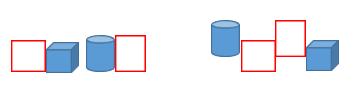
\includegraphics{colisao_quadro.png}
\caption{Exemplo de Colisão por Área de Quadrado. Não há colisão entre os dois primeiros, mas há colisão nos subsequentes}
\label{fig:colisaoQuadro}
\end{figure}

Este tipo colisão é eficaz em jogos que não necessitam de muita precisão na colisão. Objetos com áreas muito pequenas, e similares à área do quadrado também podem utilizar este modo de colisão. Seu custo de processamento é baixo.

Para casos em que há uma necessidade de maior precisão, mas não o suficiente para gerar um custo de computação, é possível se utilizar de um segundo método de colisão, a colisão por círculos, que simplesmente detecta se o círculo que contém o objeto está na área de um outro. Em jogos 3D, esse tipo de colisão é usada para objetos que não requerem muito controle de colisão, utilizando esferas no lugar de círculos.

\begin{figure}
\centering
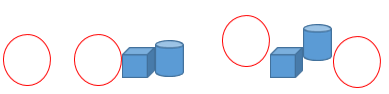
\includegraphics{colisao_esfera.png}
\caption{Exemplo de Colisão por Área de Círculo. Não há colisão entre os dois primeiros, mas há colisão nos subsequentes}
\label{fig:colisaoEsfera}
\end{figure}

Estes dois primeiros casos são suportados pela GW. São simples de implementar e possuem pouco custo. Existe uma terceira maneira, extremamente precisa, utilizada em jogos 2D (que geralmente tem seus gráficos desenhados com pixel-art), que é a Colisão de Pixels Perfeita. Este tipo de colisão lê a matriz de pixels do gráfico de ambos os objetos (não sendo necessário definir a área de colisão), e verifica, de acordo com a posição absoluta do objeto na tela, se algum dos pixels sobrescreve ao outro. Caso sim, existe uma colisão. Este tipo de colisão é custoso e não é oferecido por padrão pela GW. É possível, no entanto, estabelecer um algoritmo que simule a precisão da Colisão de Pixels Perfeita. A GW permite que se aplique várias áreas de colisão por objeto. Utilizando-se a Colisão por Quadrado, pode-se fragmentá-los para que cubram apenas a área desejada no gráfico, criando uma ilusão de Colisão de Pixels Perfeita. A desvantagem dessa abordagem é a configuração, geralmente custosa para o usuário que desenvolverá as animações, por ter que definir os quadros de colisão a cada quadro da animação.

\begin{figure}
\centering
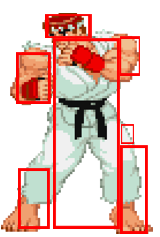
\includegraphics{multipla_colisao.png}
\caption{Exemplo de Configuração de Colisão com Múltiplos Quadrados}
\label{fig:colisaoMultipla}
\end{figure}

\subsubsection{\_\_collision\_setup(offx: number, offy: number, wd: number, hg: number, frame: number, ct: number)}

Cria uma configuração de colisão para objeto no frame especificado, com duração ct (em milissegundos), com tamanho wd x hg na posição offx vs offy. É possível criar várias caixas num mesmo frame para dar suporte ao modelo explicado acima.

\subsubsection{left() : number}

Retorna o limite mais à esquerda de todas as caixas de colisão no frame atual.

\subsubsection{right() : number}

Retorna o limite mais à dereita de todas as caixas de colisão no frame atual.

\subsubsection{top() : number}

Retorna o limite mais acima de todas as caixas de colisão no frame atual.

\subsubsection{bottom() : number}

Retorna o limite mais abaixo de todas as caixas de colisão no frame atual.

\subsubsection{colide(obj: table) : boolean}

Determina se o parâmetro obj possui caixas em colisão com as do objeto do qual a chamada foi realizada.

\subsection{Input}

Módulo responsável por controlar a entrada de eventos do controle, a fim de interagir com o jogo. Possui basicamente as entradas vermelho, verde, azul, amarelo, cima, baixo, esquerda, direita, menu, sair, sendo esses botões um padrão em controles de TVs Digitais.  Todos os métodos retornam um boolean indicando se um botão foi pressionado ou não, diferenciando-se a quantidade de vezes quando o evento é disparado.

\subsubsection{GW\_Input.pressed(key: string) : boolean}

Retorna true enquanto o botão key estiver pressionado. Útil para eventos repetitivos em jogos, como por exemplo aceleração em jogos de corrida.

\subsubsection{GW\_Input.trigger(key: string) : boolean}

Retorna true apenas no frame em que o botão key é pressionado. Se o botão continuar pressionado, retorna false continuamente até que ele seja solto. Útil para eventos não repetitivos em jogos, por exemplo, o salto de um personagem de um jogo de side-scrooling.

\subsubsection{GW\_Input.consecutive(key: string) : boolean}

Retorna true repetidamente enquanto o botão key estiver pressionado, em pequenos intervalos. 

\subsection{Utils}

Módulo agrupados de funções comuns e não associadas à classes e objetos em geral. 

\subsubsection{PROMPT(msg: string)}

Exibe a mensagem msg na tela por alguns segundos, servindo como um tipo de prompt para testes no jogo. Não deve ser utilizado para apresentar as mensagens do jogo.

\section{Aplicação de Exemplo}

Como exemplo de uso da ferramenta, será mostrado o passo-a-passo da criação de um jogo básico, um Hello World. O jogo deverá apresentar o uso das principais funcionalidades da ferramenta. Como objetivos nesse exemplo, teremos:

\begin{itemize}
  \item Apresentação de cenário de fundo e de fase;
  \item Um personagem controlado pelo controle remoto;
  \item Funcionamento de física (gravidade e colisões);
  \item Reprodução de BGM em loop.
\end{itemize}

Para programar o cenário de fundo e de fase, são necessárias duas classes diferentes. O cenário de fundo (Background) não possui interatividade com o jogador (apesar de em alguns tipos de jogos reagir a ele, como em cenários de fundo que utilizam a técnica de parallax scrolling), e, portanto é mais fácil de implementar. O cenário de fase (Base) interage com o jogador através de colisões, sendo o chão da fase. O jogador, se colidir com a face superior do cenário de fase, deve permanecer nela, não a atravessando.

O personagem de fundo deve responder ao botar vermelho do controle (ação de pular) e às setas esquerda e direita (movimento). Para programar o pulo é necessário implementar gravidade. Para a implementação de gravidade, o personagem deve ter peso, que será considerado 1. Enquanto o personagem não estiver em contato com a face superior de nenhum cenário de fase, deve receber uma aceleração negativa de -9.8m/s. Se ele pular, deve receber uma aceleração superior a 9,8 m/s a fim de alcançar uma altura desejada. A Figura \ref{fig:derExemplo} deve apresentar o diagrama de classes para o jogo de exemplo.

\begin{figure}
\centering
\makebox[\textwidth]{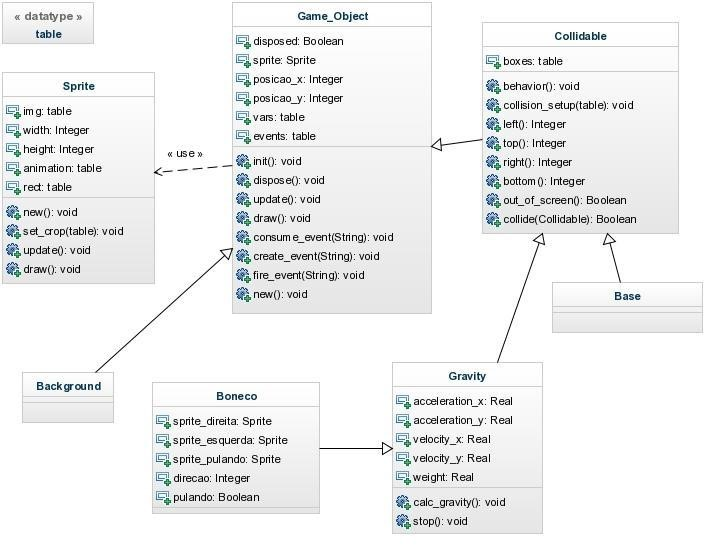
\includegraphics[width=\paperwidth-5cm]{der.jpg}}
\caption{Diagrama Entidade Relacionamento para a Aplicação de Exemplo}
\label{fig:derExemplo}
\end{figure}

Todos os objetos da cena (Background, Boneco e Base) herdam de Game\_Object, que possui os atributos básicos de um objeto de jogo. As classes Boneco e Base precisam reagir a colisões, portanto também herdam de Collidable (que por sua vez herda de Game\_Object). A classe boneco precisa reagir à gravidade, portanto herda de Gravity, que gerencia informações quanto à gravidade.

A implementação da classe Background no Código \ref{cod_ex_1}, seguido da implementação da classe Base no Código \ref{cod_ex_2}, da classe Gravity no Código \ref{cod_ex_3} e da classe Boneco no Código \ref{cod_ex_4}.

\begin{lstlisting}[caption={Classe Background},label=cod_ex_1,frame=single]
1.	GW_Codes.classes.Background = {}
2.	GW_Codes.classes.Background.superclass = "OBJECT"
3.	function GW_Codes.classes.Background:init()
4.		GWClasses.Background.__superClass().init(self)
5.		self.sprite = 
		Sprite.new('/backgrounds/back1.png')
6.	end
\end{lstlisting}

\begin{lstlisting}[caption={Classe Base},label=cod_ex_2,frame=single]
1.	GW_Codes.classes.Base = {}
2.	GW_Codes.classes.Base.superclass = "COLLIDABLE"
3.	function GW_Codes.classes.Base:init()
4.		GWClasses.Base.__superClass().init(self)
5.		self.sprite = 
		Sprite.new('/characters/base.png')
6.		self.pos.x = 0
7.		self.pos.y = 600-33
8.		self.vars.__collision_data.loop = true
9.		self:__collision_setup(0,0,800,33,100)
10.	end
\end{lstlisting}

\begin{lstlisting}[caption={Classe Gravity},label=cod_ex_3,frame=single]
1.	GW_Codes.classes.Gravity = {}
2.	GW_Codes.classes.Gravity.superclass = "COLLIDABLE"
3.	function GW_Codes.classes.Gravity:init()
4.		GWClasses.Gravity.__superClass().init(self)
5.		self.vars.accy = 0.0
6.		self.vars.accx = 0.0
7.		self.vars.velx = 0.0
8.		self.vars.vely = 0.0
9.		self.vars.weight = 1.0
10.	end
11.
12.	function GW_Codes.classes.Gravity:calc_gravity()
13.		local add_accel = { 
			x = Game_Timer:sync(self.vars.accx), 
			y = Game_Timer:sync(self.vars.accy) } 
14.		self.vars.velx = self.vars.velx + add_accel.x
15.		self.vars.vely = self.vars.vely + add_accel.y
16.		self.pos.x = self.pos.x + self.vars.velx
17.		self.pos.y = self.pos.y + self.vars.vely
18.	end
\end{lstlisting}

\begin{lstlisting}[caption={Classe Boneco},label=cod_ex_4,frame=single]
1.	GW_Codes.classes.Boneco = {}
2.	GW_Codes.classes.Boneco.superclass = "Gravity"
3.	function GW_Codes.classes.Boneco:init()
4.		GWClasses.Boneco.__superClass().init(self)
5.		self.vars.sprites = {}
6.		self.vars.sprites.d = 
		Sprite.new('/characters/mario_parado.png')
7.		self.vars.sprites.e = 
		Sprite.new('/characters/mario_parado_m.png')
8.		self.sprite = self.vars.sprites.d
9.		self.pos.x = 800/2-16
10.		self.pos.y = 16
11.		self.vars.weight = 2.5
12.		self.vars.lado = 'd'
13.		self.vars.__collision_data.loop = true
14.		self:__collision_setup(9,7,15,19,100)
15.	end
16.
17.	function GW_Codes.classes.Boneco:behavior()
18.		GWClasses.Boneco.__superClass().behavior(self)
19.		local vel = 5.0
20.		self.vars.velx = 0.0
21.		if GW_Input.pressed('CURSOR_RIGHT') then
22.			self.sprite = self.vars.sprites.d
23.			self.vars.velx = vel
24.		end
25.		if GW_Input.pressed('CURSOR_LEFT') then
26.			self.sprite = self.vars.sprites.e
27.			self.vars.velx = -vel
28.		end
29.		local tempx = Game_Timer:sync(self.vars.velx)
30.		self.pos.x = self.pos.x + self.vars.velx
31.	end
\end{lstlisting}

As classes Background e Base são estáticas na tela, portanto é seguro aplicar-lhes um posicionamento estático por toda a vida da aplicação.

Tendo sido implementadas as classes de funcionamento básico do jogo, podemos passar para a criação da Scene que irá gerenciar a lógica e recursos. Será dever da Scene instanciar e destruir objetos, invocar BGMs, determinar o fluxo da lógica (muitas vezes chamada de Máquina Finita de Estados), etc. A GW provê uma Scene já pronta para uso, ela não deve ser instanciada. Em casos da necessidade do uso de mais de uma Scene, o ideal é a implementação de uma nova classe que desempenhe a função, sendo controlada pela Scene provida pela GW.

No caso da aplicação de exemplo, a Scene vai instanciar o Backgroun, a Base e o Boneco. Vai tocar uma BGM em modo infinito (loop) e vai gerenciar os eventos disparados pela interação dos objetos. O código segue no Código \ref{cod_ex_5}.

\begin{lstlisting}[caption={Código da Cena},label=cod_ex_5,frame=single]
1.	function GWScene:begin()
2.		print("cena inicializada")
3.		self.vars.background = 
		GWClasses['Background'].new()
4.		self.vars.mario = GWClasses['Boneco'].new()
5.		self.vars.base = GWClasses['Base'].new()
6.		table.insert(self.objects, self.vars.background)
7.		Game_Graphics:
		insertLayer(1, self.vars.background)
8.		table.insert(self.objects, self.vars.base)
9.		Game_Graphics:insertLayer(1, self.vars.base)
10.		table.insert(self.objects, self.vars.mario)
11.		Game_Graphics:insertLayer(2, self.vars.mario)
12.		Game_Resources.play_BG('playback', true)
13.		self.vars.gravity = 9.8
14.	end
15.
16.	function GWScene:behavior()
17.		local mario = self.vars.mario 
18.		if mario:right() >= Game_Graphics.width then
19.			mario.pos.x = Game_Graphics.width - 
		(mario:frame().offset.x + mario:frame().width) 
20.		end
21.		if mario:left() <= 0 then
22.			mario.pos.x = -mario:frame().offset.x 
23.		end
24.		mario:calc_gravity()
25.		if mario:collide(self.vars.base) then
26.			mario.vars.accy = 0.0
27.			mario:stop()
28.			mario.pos.y = self.vars.base:top() - 
			(32-7)
29.		else 
30.			if mario.vars.accy < 0 then
31.				mario.vars.accy = 
			mario.vars.accy + self.vars.gravity
32.			else
33.				mario.vars.accy = 
				self.vars.gravity
34.			end
35.		end
36.		if GW_Input.pressed('CURSOR_UP') and 
			mario:collide(self.vars.base) then
37.			mario.vars.accy = mario.vars.accy - 
			self.vars.gravity * 5
38.		end
39.	end
\end{lstlisting}

As linhas 2-11 criam os objetos na cena e os registram junto à Scene e ao módulo de gráficos (Game\_Graphics). O registro com o Game\_Graphics permite que o módulo reconheça os objetos como desenháveis e vai invocar o método draw() de cada objeto registrado para que apareça na tela. A linha 12 faz com que a BGM playback seja tocada. Na linha 13, setamos a gravidade global para o valor 9,8 (m/s).

Na função behavior o objeto mario (Boneco) tem sua gravidade setada para a global. Da linha 18-23 é feito o tratamento para quando o objeto tentar sair da tela pelos lados. Nas linhas 25-35 é feito o tratamento para quando o objeto colide com a base. As linhas 36-38 tratam o pulo do boneco, adiciona aceleração negativa (assim ele irá para cima).

Com a Scene pronta, é necessário agora configurar os sons. A configuração do som exige que se utilize o módulo Parameters. A GW não tem como tocar sons nativamente, nem saber sua duração. Serão utilizados parâmetros para se informar esses dados através do NCL. Apenas uma sobrescrita da função parse é necessária, como mostrado no Código \ref{cod_ex_6}.

\begin{lstlisting}[caption={Código dos Parâmetros},label=cod_ex_6,frame=single]
1.	function GWInitializer:parse(id,par)
2.		if string.match(par, "BGM%d+") ~= nil then
3.			print("Registering BGM "..id)
4.			local duracao = 
			string.match(par, "BGM(%d%d%d%d)")
5.			local minutos = 
			tonumber(string.sub(duracao, 0, 2))
6.			local segundos = 
			tonumber(string.sub(duracao, 3))
7.			Game_Resources.
			register_sound(id, 
				minutos * 60 + segundos)
8.		end
9.		if par == "End" then
10.			print("BGM "..id.." ended")
11.			Game_Resources.end_BG(id)
12.		end
13.	end
\end{lstlisting}

Nesta implementação, a função recebe um parâmetro informando o id da mídia no NCL e sua duração no parâmetro par. A GW reconhece que é um som caso contenha a palavra BGM seguido de 4 inteiros, que representam a duração do som em minutos e segundos. Essa duração é utilizada para saber quando o som terá terminado e mandar tocar de novo. Para que funcione, é preciso que o NCL disponibilize links para inicializar e finalizar uma mídia de som. 
Todo o trabalho do lado do código Lua está pronto. Agora é necessário criar o código NCL que irá invocar e parametrizar a aplicação Lua. O código segue nos Códigos \ref{cod_ex_7} e \ref{cod_ex_8}.

\begin{lstlisting}[caption={Regiões e Descritores de Exemplo},label=cod_ex_7,frame=single]
<!-- Regioes -->
<regionBase>
    <region id="screen" width="100%" height="100%"  zIndex="5"/>
    <region id="music" width="100%" height="100%" zIndex="0"/>
</regionBase>
<!-- Descritores -->
<descriptorBase>
    <descriptor id="dsScreen" region="screen" focusIndex="240"/>
    <descriptor id="dsMusic" region="music">
        <descriptorParam name="soundLevel" value="1"/>
    </descriptor>                
</descriptorBase>
\end{lstlisting}

\begin{lstlisting}[caption={Portas, Medias e Links},label=cod_ex_8,frame=single]
<!-- Porta -->
<port id="entryPoint" component="lua"/>
<media id="lua" src="codes/main.lua" descriptor="dsScreen">
    <property name="start1"/>
    <property name="playback"/>
</media>
<media id="playback" type="audio/mp3" 
	src="media/backtracks/teste.mp3"/>
<media id="programSettings" type="application/x-ginga-settings">
    <property name="service.currentKeyMaster" value="240"/>
</media>
<!-- DEFINICAO DOS LINKS AQUI!!!!!!!! -->
<link xconnector="onBeginSetN">
    <bind role="onBegin" component="lua" />
    <bind role="set" component="lua" interface="start1"/>
    <bind role="set" component="lua" interface="playback">
        <bindParam name="var" value="BGM0036"/>                
    </bind>
</link>
<link xconnector="onEndAttributionStart">
    <bind role="onEndAttribution" component="lua" 
    	interface="playback" />
    <bind role="start" component="playback" />
</link>
\end{lstlisting}

É criada a mídia playback com o som a ser reproduzido. São inseridas propriedades na mídia Lua, que tem finalidades específicas: a propriedade start1 informa à GW que ela deve esperar por 1 parâmetro pelo menos (além do próprio start1). Isso ocorre porque a passagem de parâmetros entre o NCL e o Lua não segue a ordem estabelecida no código XML e em alguns casos, quando há muitos links, alguns deixam de ser enviados. O parâmetro playback será o id do som na GW. Este parâmetro deve ser setado com o valor BGM0036. Como dito acima, BGM diz à GW (neste exemplo) que o parâmetro é um som, enquanto que 0036 informa que o som tem a duração de 0 minutos e 36 segundos. Com esta configuração, está pronta o Hello World da GW, apresentado nas Figuras \ref{fig:imgEx1}, \ref{fig:imgEx2} e \ref{fig:imgEx3}.

\begin{figure}
\centering
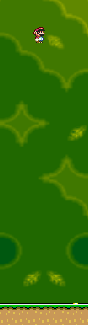
\includegraphics{img_ex_1.png}
\caption{Boneco em Queda Livre}
\label{fig:imgEx1}
\end{figure}

\begin{figure}
\centering
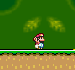
\includegraphics{img_ex_2.png}
\caption{Boneco em Repouso na Base}
\label{fig:imgEx2}
\end{figure}

\begin{figure}
\centering

\includegraphics{img_ex_3.png}
\caption{Boneco durante Salto}
\label{fig:imgEx3}
\end{figure}


\chapter{Estudo de Caso: Tetris}

A fim de testar a capacidade da engine, este capítulo apresenta um estudo de caso de um jogo, nominamente, uma versão de Tetris implementada para TVi. Um jogo, sendo uma aplicação de hipermídia, envolve diversas formas de se comunicar com o usuário. Jogos se utilizam de gráficos, efeitos sonoros, jogabilidade e narrativa para se comunicar com o jogador. Para oferecer todos estes tipos de mídia é necessário hardware capaz de processar esse tipo de dado. O STB em geral (modelos econômicos) não possuem muito poder de hardware, não tendo como função executar aplicações pesadas e/ou complexas. É preciso, portanto, analisar a capacidade de processamento da STB em relação ao jogo para averiguar se o hardware é capaz de entregar uma taxa de frames razoável. A jogabilidade deve ser avaliada através de uma análise da ergonomia e resposta do controle remoto (meio principal de entrada de dados no STB). Controles não foram designados para responder a múltiplos comandos simultâneos, portanto os jogos precisam ser viáveis recebendo uma única entrada de cada vez. Por fim, deve-se analisar qual é o público alvo para o jogo. A maioria da população disposta a jogar jogos casuais o farão utilizando o telefone celular. Para que algum jogo possa ter sucesso em uma TV Digital, é preciso realizar um estudo da população disposta a jogar na TV Digital e o que eles esperam em um jogo. Todos esses fatores influenciam na escolha de um jogo de sucesso na TV Digital utilizando a STB.

Realizar uma triagem do anseio da população disposta a jogar em uma TV Digital está fora do escopo deste trabalho, portanto apresentaremos um jogo pioneiro na história dos jogos, comumente utilizado como aplicação de teste em engines de games por sua (deveras) simplicidade e fama: Tetris.

\section{Limitações do Set-Top Box}



\section{Tetris}

\subsection{História}

While working for the Computing Center at the Academy of Sciences of the USSR, Alexey Pajitnov envisions an electronic game in which players could arrange puzzle pieces in real time while they fell from the top of the playing field at increasing speeds. Using an Electronika 60 computer, he designs a game that features seven distinctive geometric game pieces, each made up of four squares. Alexey calls the game “Tetris,” a combination of the word “tetra” (Greek word meaning “four”) and “tennis” (his favorite sport). The game is ported to the IBM PC and becomes an immediate hit with his colleagues, spreading like wildfire throughout the Soviet Union.

Tetris begins its global expansion by launching on PCs in North America and Europe. The game is showcased at the 1988 Consumer Electronics Show in Las Vegas, where Henk Rogers, video game designer and publisher, comes across it and gives Tetris a try. He’s immediately hooked and thinks there’s something special about the game (he wasn’t wrong!). His company, Bullet-Proof Software, obtains the rights to releases Tetris for PC and NES in Japan, and more than 2 million copies are sold.

Henk meets Alexey, and the two immediately click and become close friends. When Henk secures the handheld rights to Tetris and licenses the rights to Nintendo, the successful video game company bundles Tetris with its new Game Boy portable gaming console. This perfect pair results in the sales of a whopping 35 million copies!

A university’s scientific research suggests that practicing Tetris can help the brain operate more efficiently. It’s no wonder why Russian cosmonaut Aleksandr A Serebov decides to take his Nintendo Game Boy and Tetris game cartridge aboard the Soyus TM-17 rocket en route to the MIR Space Station. He spends 197 days working in the station and helps Tetris become the first video game in space!

Henk establishes Blue Planet Software, Inc. as the exclusive agent for the Tetris brand. Shortly after, The Tetris Company is formed, becoming the source of all licenses to Tetris. Many aspects of the game become standardized and, with the help of artist Roger Dean, a bold and distinctive Tetris logo is created.

G-mode publishes a mobile Tetris game, boosting it to Japan’s #1 spot in games for mobile phones! To continue the development of Tetris for mobile devices, Henk establishes Blue Lava Wireless, and Tetris rapidly gains momentum in the North American mobile market. Eventually, Jamdat purchases Blue Lava Wireless and obtains an exclusive license to publish Tetris on mobile devices.

EA obtains Jamdat and becomes the new exclusive licensee of Tetris for mobile devices. Meanwhile, Nintendo releases Tetris for the DS and sells over two million copies worldwide!  As he watches the global impact of his creation continue to grow, Alexey receives the “First Penguin Award” at the Game Developers Conference, where Tetris is widely recognized as the game that gave birth to the casual game industry.

EA Mobile releases Tetris for the iPhone and iPod touch platforms, while Tetris Online releases Tetris Party for Nintendo Wii. Tetris Party quickly climbs to the #1 spot for WiiWare downloads and nominated for “Best WiiWare Game 2008” and “Best Puzzle Game 2008” by IGN.

Happy 25th anniversary! Tetris Online unveils the first official web-based Tetris game site, Tetris Friends Online Games. The website is a success, and more good news rolls in as Tetris ranks #2 in the “Top 50 Console Games of All Time,” according to the Guinness World Records 2009 Gamer’s Edition.

Without skipping a beat, a new Tetris app for iPad debuts, Tetris Party Deluxe is released for Nintendo Wii and DS, Tetris for PlayStation Network launches to critical acclaim, and a new Tetris line of lifestyle merchandise is introduced worldwide. To top off the year, Tetris surpasses 100 million paid mobile downloads, becoming the best-selling mobile game of all time!

Tetris is named PlayStation Network’s #1 game, while the launch of Tetris Axis for Nintendo 3DS initiates the game’s expansion into augmented reality. This year also marks the release of the Tetris board game, Tetris Link, which brings Tetris off of the screen and onto your table! Tetris Link receives several awards, including American Mensa’s “Mensa Select Award,” Toy of the Year Award’s “Game of the Year,” and Good Housekeeping Research Institute’s “Best Game of 2011.”

\subsection{Regras de Tetris}

As regras no jogo tetris se definem como especificado a seguir. O site oficial de Tetris não especificam as regras do jogo, e portanto essas regras citadas a seguir foram extraídas através da experiência os jogadores.

O jogo acontece dentro de uma máquina, chamada Tétrion. O Tétrion é formado de dez espaços horizontais e 20 verticais, onde se pode mover os tetraminós. Tetraminós escolhidos aleatoriamente caem do topo do Tétrion, um de cada vez. Cada tetraminó entra no campo com uma orientação e cor dependente de seu formato. Parte do Tétrion, chamada \textit{piece preview}, mostra as próximas peças que irão entrar em campo.

O jogador pode rotacionar o tetraminó que está caindo em noventa graus, considerando que haja espaço para que a peça rotacione. Algumas versões do jogo ajustam a posição do tetraminó para que ele consiga realizar a rotação.

O jogador pode movimentar o tetraminó para os lados (um espaço por vez), considerando que haja espaço para que a peça se mova. As peças não podem ultrapassar paredes ou outros blocos.

No topo-esquerda, ou em outros casos, no fundo-direita do Tétrion, pode existir uma área chamada \textit{hold box}, onde o jogador pode armazenar um tetraminó para uso no futuro. A qualquer momento, enquanto um tetraminó cai, o jogador pode movê-lo para a \textit{hold box}, fazendo com que o tetraminó armazenado seja levado ao topo do Tétrion.

Cada tetraminó se move para baixo, devagar. Geralmente, o jogador pode usar algum método para "derrubar" o tetraminó, ou fazê-lo se mover mais rápido para baixo. Quando a peça cai no chão ou em outras peças, ela irá aguardar um pouco antes de se fixar ao campo. Durante este tempo o jogador poderá ainda movê-lo para tentar encaixá-lo em algum lugar. Depois de fixo, o jogador já não pode mover mais o tetraminó.

Quando o tetraminó se fixa e preenche todo o espaço de uma linha, esta linha irá ser limpa (as peças na linha, removidas). Os blocos acima da linha irá se mover para baixo, de acordo com a quantidade de linhas preenchidas.

Se o campo não estiver preenchido com blocos, a próxima peça entra. Se o tetraminó não puder ser alocado no campo, pelo menos parcialmente, devido às regras acima, é considerado fim de jogo.

\subsection{Diretrizes}

A partir da criação da empresa Tetris Company, foi criada uma diretriz para que todos os jogos lançados posteriormente mantivessem um padrão de jogabilidade. Essas diretrizes, assim como as regras, não estão disponíveis oficialmente e foram inferidas através da experimentação dos jogadores.

\begin{itemize}
  \item Campo de jogo do Tétrion tem tamanho de 10x22 células, sendo as linhas acima da 20ª ocultas (servem para inserir tetraminós parcialmente no campo).
  \item Cores dos tetraminós
  \begin{itemize}
  	\item I: ciano
  	\item O: amarelo
  	\item T: roxo
  	\item S: verde
  	\item Z: vermelho
  	\item J: azul
  	\item L: laranja
  \end{itemize}
  \item As peças I e O aparecem nas colunas centrais
  \item As outras aparecem guidas mais à esquerda
  \item Os tetraminós aparecem em formato horizontal, com a parte plana apontada para baixo
  \item O \textit{Super Rotation System} (SRS) especifica a rotação do tetrominó
  \item Standard mappings for console and handheld gamepads:
  \begin{itemize}
   	\item Up, Down, Left, Right on joystick perform locking hard drop, non-locking soft drop (except first frame locking in some games), left shift, and right shift respectively.
   	\item Left fire button rotates 90 degrees counterclockwise, and right fire button rotates 90 degrees clockwise.
   	\item Purple T
   	\item Green S
   	\item Red Z
   	\item Blue J
   	\item Orange L
  \end{itemize}
  \item Standard mappings different from console/handheld gamepads for computer keyboards
  \item So-called Random Generator (also called "random bag" or "7 system")
  \item "Hold piece": The player can press a button to send the falling tetromino to the hold box, and any tetromino that had been in the hold box moves to the top of the screen and begins falling. Hold cannot be used again until after the piece locks down. Games on platforms with fewer than eight usable buttons (such as the version on iPod) may skip this feature. The combination of hold piece and Random Generator would appear to allow the player to play forever.
  \item Game must have ghost piece function.
  \item Terms used in the user manual: "Tetriminos" not "tetrominoes" nor "tetrads" nor "pieces", letter names not "square" nor "stick", etc.
  \item Designated soft drop speed. Details vary between guideline versions.
  \item Player may only level up by clearing lines or performing T-Spin. Required lines depends in the game.
  \item The game must use a variant of Roger Dean's Tetris logo, although this was true from around 2000 - before the guidelines emerged.
  \item Game must include a song called Korobeiniki. (Guideline 2005~)
  \item The player tops out when a piece is spawned overlapping at least one block, or a piece locks completely above the visible portion of the playfield.
\end{itemize}

The extent to which the Guideline specifies the speed curve, the scoring system, and other aspects not listed on this page, is not yet known to the public.

Although Guideline-compliant games share many traits, they also have differences in many aspects as well. There are a few instances where a game will break a trait which is shared by all other games thought to be compliant. Examples of this include the lack of the hold function and the T-spin's ability to start and continue Back-to-Back chains in iPod Tetris, and the inverted rotation button layout of TGM3 and TGM ACE (or Kiwamemichi, depending on interpretation). No explanations have been given for the reasons of these games' deviations.

Super Rotation System, or SRS is the current Tetris Guideline standard for how tetrominoes behave, in a broad sense. SRS represents where and how tetrominoes spawn, how they rotate, and what wall kicks they may perform. In TI, a player may choose between World and Classic rotation styles. World closely resembles SRS, and Classic closely resembles the rotation styles of its predecessors TGM and TAP. Henk Rogers, in his effort to unify all new Tetris games into the Tetris Guideline, required Arika to include SRS, which is called World in Ti. SRS traces its routes back to 1991 when BPS introduced its signature third and fourth orientations for the S, Z, and I tetrominoes in their Tetris 2+Bombliss. Later would come flipped-side-up spawned T, L, and J tetrominoes and flexible new wall kicks. Probably the most accurate SRS finds itself in BPS's latest games Tetris Worlds and Tetris Deluxe, which both feature exact same rotation styles.

All tetrominoes exist inside a bounding square and rotate about the center of this square unless obstructed. Tetrominoes of width 3 (J, L, S, T, Z) are placed in the top two rows of the bounding square and (for J, L, and T) with the flat side down. I is placed in the top middle row.

All tetrominoes spawn in 2 usually hidden rows at the top of the playfield. They are placed in the center of these rows, rounding to the left.

Once a tetromino lands, it does not lock until the lock delay expires. The lock delay behavior, called Infinity by the Tetris Company, resets the lock delay whenever the tetromino is moved or rotated. Hard drop is generally mapped to up, which has no lock delay.

Wall kicks in SRS are extremely flexible compared to those of earlier games. Some rotations result in new positions that do not overlap the former position at all, allowing for highly controversial T-spin triples (see Twist).

The Random Generator is BPS's name for the algorithm used to generate the sequence of tetrominoes in Tetris brand games that follow the Tetris Guideline.

Random Generator generates a sequence of all seven one-sided tetrominoes (I, J, L, O, S, T, Z) permuted randomly, as if they were drawn from a bag. Then it deals all seven tetrominoes to the piece sequence before generating another bag. There are 7!, or 5,040, permutations of seven elements, and it is believed that Tetris assigns a nearly equal probability to each of these, making it much less likely that the player will get an obscenely long run without a desired tetromino. It can produce a maximum of 12 tetrominoes between one I and the next I, and a run of S and Z tetrominoes is limited to a maximum of 4. Exception: In Random Generator as implemented in Tetris The Grand Master Ace, the first piece of the first bag is always I, J, L, or T, just as in the traditional TGM randomizer.

Despite the generic sounding name, presumed employees of BPS are known to treat the term "Random Generator" as a unique name, referring only to this particular algorithm.

While the number of tetrominoes in a single bag is usually 7, some games use a different number. The public beta of Tetris Online (Japan) used an 8-bag randomizer for the player. Not all guideline-compliant games use the Random Generator in all modes. Tetris Worlds and Tetris Green, for instance, use a different randomizer in their Square modes, and TGM3 uses the TGM randomizer even when the game is set to "World" mode.

There are two "snake" tetrominoes, called S and Z. As only two snakes will be in a given bag, a sequence of more than two snakes must cross the "seam" between bags. The probability of the next two bags having a sequence of four consecutive snakes, the maximum possible, is 1/(7*6*7*6) for SZSZ and likewise for SZZS, ZSSZ, and ZSZS, for a total of 1/441. But the probability of these being your three next pieces are 1/441 times the probability of being at position 6 in a bag, so the probability of the next four pieces being SZSZ are 1 in 3087.

Define a "2|1 combo" as chosen sixth and seventh pieces in one bag and first piece in next bag, and a "1|2 combo" as chosen seventh piece in one bag and first and second pieces in next bag. Define a "snake" as the S tetromino or the Z tetromino.

The probability of any 2|1 combo (e.g. SZ|Z) is 1/(7*6*7) = 1/294. There are four different 2|1 combos containing all snakes (SZ|Z, SZ|S, ZS|Z, and ZS|S), so the probability of getting a 3-snake 2|1 in your next two bags is 4/294. But the probability of being at the sixth piece in a bag, where your next three pieces are a 2|1, is 1/7, making the probability of being at a three-snake 2|1 equal to 4/(294*7) = 2/1029. By symmetry, the 1|2 probabilities are exactly the same: 2/1029. So for Random Generator, this makes a 1 in 257 chance of your next three tetrominoes being snakes.

The Ghost piece, or ghost for short, also called shadow or (in Arika games) Temporary Landing System (TLS), is a representation of where a tetromino or other piece will land if allowed to drop into the playfield. It is generally colored fainter than the falling piece and the blocks in the playfield. As the player moves the falling piece, the ghost piece moves below it; when the piece falls far enough that it overlaps the ghost piece, the falling piece is always drawn in front.

Older games did not have a ghost piece, but all games that conform to the Tetris Guideline allow the player to use a ghost piece at all times, and Dr. Mario for Nintendo 64 has a ghost piece as well. The ghost piece reduces the number of misdrops, especially for beginners or for high-speed players who use hard drop, but some players who are migrating from games without a ghost piece have trouble adjusting to the ghost piece when they fail to distinguish it from blocks in the playfield.

\section{Documentação da Aplicação}



\section{Resultados}

\chapter{Conclusões} 

\end{document}